\appendix
\begin{frame}
\tableofcontents[currentsection]
\end{frame}


\begin{frame}
\begin{columns}
    \begin{column}{.4\textwidth}
        \begin{figure}
            \centering
            \def\stackalignment{r}
            \stackunder{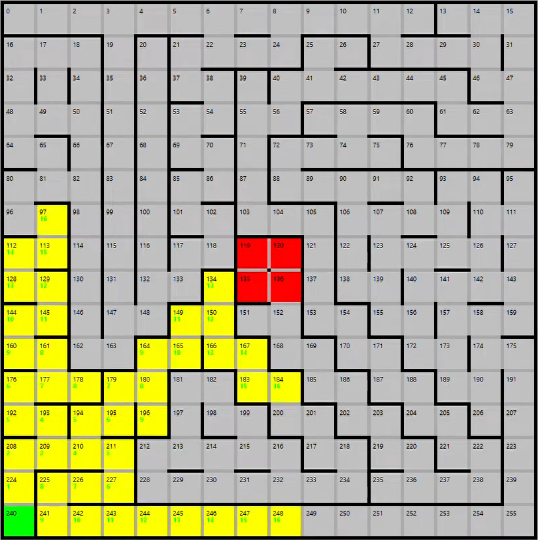
\includegraphics[width=0.9\linewidth]{assets/floodfill.png}}%
               {\sources
                Source: \url{github.com/lime7git/micromouse}}
        \end{figure}
    \end{column}
    \begin{column}{.7\textwidth}
        \begin{itemize}
            \item Algorithme de floodfill (parcours en largeur)
            \item Les chemins sont tracés pour suivre les milieux des cases
            \item Pour les géométries très particulières telles que dans le cas des labyrinthes \textit{Micromouse}.
        \end{itemize}
    \end{column}
\end{columns}
\end{frame}


\begin{frame}
\begin{proof}[Preuve de la complexité de l'algorithme de Fortune]
    Il y a \(n\) sites, et un nombre d'évènements cercles en \(O(n)\). Le traitement d'un évènement est en \(O(\log n)\) (Ajout, retrait, recherches dans des tas et arbres équilibrés). D'où une complexité en \(O(n\log n)\).\\
    \vspace{1em}
    Optimalité : Un diagramme de Voronoï permet de trier \(n\) réels, la complexité en \(O(n\log n)\) est donc optimale.
\end{proof}
\end{frame}


\begin{frame}{Quelques bizarreries}
\begin{figure}
    \centering
    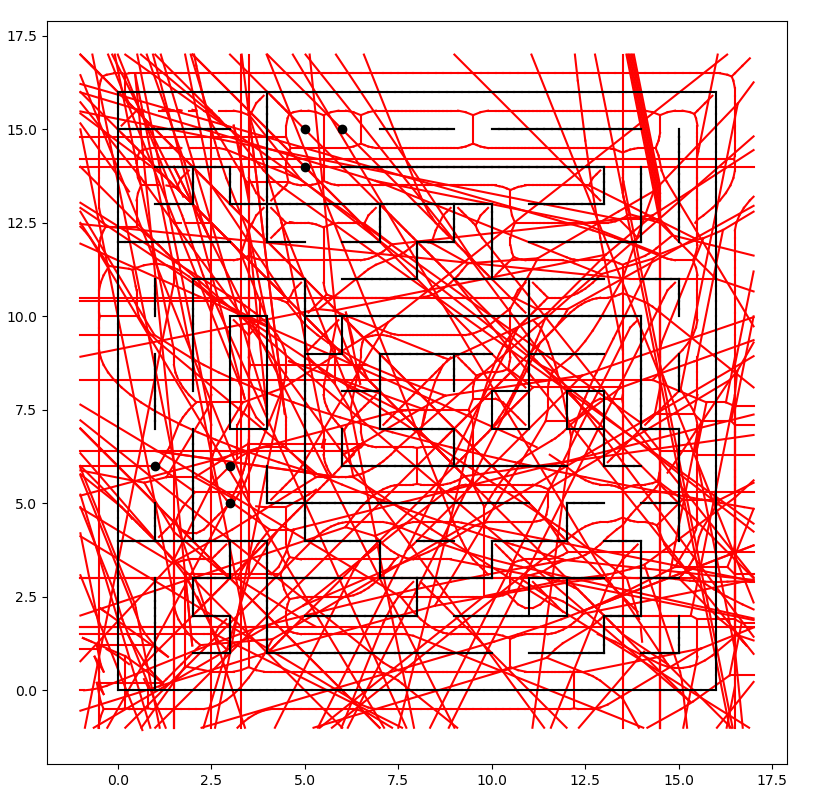
\includegraphics[width=0.6\linewidth]{assets/Bizarre.png}
\end{figure}
\end{frame}

%%%%%%%%%%%%%%%%%%%%%%%%%%%%%%
% A* PYTHON
%%%%%%%%%%%%%%%%%%%%%%%%%%%%%%
\begin{frame}[fragile]
\begin{code}
\begin{minted}[fontsize=\codesize]{python}
def a_star(self, heuristique: Callable, depart: tuple, arrivee: tuple):

    queue = PriorityQueue()
    queue.put((0, (i_dep, j_dep))) # Initialisation de la file de priorité avec le départ

    parents = {}
    longueur_plus_court_chemin = {}
    longueur_plus_court_chemin[(i_dep, j_dep)] = 0

    while not queue.empty():
        _, point = queue.get() # On enlève le minimum
        i, j = point
        if point == (i_arr, j_arr):
            return reconstituer_chemin() # On est arrivé, on reconstruit le chemin

        for voisin in CarteNaif.voisins_points(i, j):
            if voisin not in self.matrice or
            self.dist_obstacle[voisin] < Settings.NAIF_MARGE:
                continue
            tentative_chemin = longueur_plus_court_chemin[point] + # Potentiel meilleur chemin
                Point.distance_eucli(i, j, *voisin)                # trouvé jusqu'à voisin
            if voisin not in longueur_plus_court_chemin or
            tentative_chemin < longueur_plus_court_chemin[voisin]:
                parents[voisin] = point
                longueur_plus_court_chemin[voisin] = tentative_chemin
                meilleure_heuristique = tentative_chemin +
                    heuristique(voisin, (i_arr, j_arr))
                queue.put((meilleure_heuristique, voisin))

    raise CheminNonTrouve("Chemin naïf non trouvé")
    

\end{minted}
\end{code}
\end{frame}

%%%%%%%%%%%%%%%%%%%%%%%%%%%%%%
% DCEL PYTHON
%%%%%%%%%%%%%%%%%%%%%%%%%%%%%%
\begin{frame}[fragile]
\begin{code}
\begin{minted}[fontsize=\codesize]{python}
class HalfEdge:

    def __init__(self, point_incident: Point, jumelle: "HalfEdge" = None, origine: Vertex = None):

        # Pointeur vers l'origine de l'arête
        self.origin = origine

        # Le point dont l'arête est incidente (ie. le point de la cellule de Voronoi)
        self.point_incident = point_incident

        # L'autre arête incidente sur le même point (dans le sens contraire)
        self._jumelle = None
        self.jumelle = jumelle

        # Suivant et précédent
        self.suiv = None
        self.prec = None
\end{minted}
\end{code}
\end{frame}


%%%%%%%%%%%%%%%%%%%%%%%%%%%%%%
% Filtrage arêtes PYTHON
%%%%%%%%%%%%%%%%%%%%%%%%%%%%%%
\begin{frame}[fragile]
\begin{code}
\begin{minted}[fontsize=\codesize]{python}
@classmethod
def from_voronoi(cls, voronoi: Voronoi, carte_origine: Carte) -> 'CarteGraphee':

    sites: List[Point_V] = list(voronoi.sites)
    aretes: List[HalfEdge] = voronoi.edges
    vertices: List[Vertex] = voronoi.vertices

    def vertex_to_tuple(vertex: Vertex): ...
    def point_to_tuple(p: Point): ...
    def pointV_to_tuple(p: Point_V): ...
    def est_meme_obstacle(p1: Point_V, p2: Point_V): ...

    ...

    carte: CarteGraphee = cls(carte_origine)
    
    for e in aretes:
        center: Point_V = e.point_incident
        point_oppose: Point_V = e.jumelle.point_incident
        if point_oppose is not None:
            d = Point.distance_eucli(
                center.xd, center.yd, point_oppose.xd, point_oppose.yd)
            if d >= Settings.MULT_ESPACEMENT_SITES * Settings.PRECISION and not 
            (carte_origine.obstacles_convexes and est_meme_obstacle(center, point_oppose)):
    
                carte.ajouter_arete((source := vertex_to_point[vertex_to_tuple(e.origine)]), (
                    dest := vertex_to_point[vertex_to_tuple(e.cible)]), source.distance(dest))
    
    return carte
\end{minted}
\end{code}
\end{frame}


\begin{frame}[fragile]
\begin{code}
\begin{minted}[fontsize=\codesize]{python}
@classmethod
def from_scratch(cls, nom_fichier: str, bounding_size: Tuple, force_bound: bool) -> 'CarteGraphee':

    carte_raw: Carte = Carte.lire_carte(nom_fichier)
    (x_min, x_max), (y_min, y_max) = bounding_size
    if force_bound:
        carre = [
            Point(x_min, y_min),
            Point(x_min, y_max),
            Point(x_max, y_max),
            Point(x_max, y_min)
        ]
        carte_raw.obstacles.append(Obstacle(carre, False, True))
    carte_raw.decouper_obstacles(Settings.PRECISION) # Découpage des obstacles
    bounding_box = BoundingBox(x_min, x_max, y_min, y_max)
    v = Voronoi(bounding_box) # Création du diagramme de Voronoi
    v.creer_diagramme(points=list(carte_raw.voronoi_set()))

    carte: CarteGraphee = cls.from_voronoi(v, carte_raw) # Extraction de la carte simplifiée
    carte.simplifier_graphe()
    # carte.supprimer_culs_de_sac()
    return carte
\end{minted}
\end{code}
\end{frame}


\begin{frame}[fragile]
\begin{code}
\begin{minted}[fontsize=\codesize]{python}
def creer_diagramme(self, points: list):

    self.initialiser(points) # Initialiser tous les points
    index = 0
    premier_point = None

    while not self.event_queue.empty():

        event = self.event_queue.get() # Retirer l'event de plus petite priorité
        premier_point = premier_point or event.point

        # Traitement des circle event
        if isinstance(event, CircleEvent) and event.est_valide:
            self.sweep_line = event.yd # Mise à jour sweep line
            self.traitement_circle_event(event)

        # Traitement des site event
        elif isinstance(event, SiteEvent):
            event.point.nom = index
            index += 1
            self.sweep_line = event.yd # Mise à jour sweep line
            self.traitement_site_event(event)
        else: continue

        self.event = event

    # Finalisation avec la bounding box
    self.edges = self.bounding_poly.finish_edges(
        edges=self.edges, vertices=self._vertices, points=self.sites, event_queue=self.event_queue
    )
\end{minted}
\end{code}
\end{frame}


\begin{frame}[fragile]
\begin{code}
\begin{minted}[fontsize=\codesize]{python}
def traitement_site_event(self, event: SiteEvent):

    # Créer un nouvel arc
    point_i = event.point
    new_arc = Arc(origine=point_i)
    self._arcs.add(new_arc)

    # 1. Si la ligne de front est vide, on insère le point.
    if self.arbre_front is None:
        self.arbre_front = NoeudFeuille(new_arc)
        return

    # 2. Recherche de l'arc au dessus du points
    arc_node_above_point = Arbre_AVL.chercher_noeud_feuille(self.arbre_front, cle=point_i.xd, sweep_line=self.sweep_line)
    arc_above_point = arc_node_above_point.get_value()

    # Retirer une potentielle fausse alerte
    if arc_above_point.circle_event is not None:
        arc_above_point.circle_event.fausse_alerte()

    # 3. Remplacer la feuille par le nouveau sous-arbre représentant les deux nouvelles intersections
    point_j = arc_above_point.origine
    breakpoint_gauche = Breakpoint(breakpoint=(point_j, point_i))
    breakpoint_droite = Breakpoint(breakpoint=(point_i, point_j))

    root = NoeudInterne(breakpoint_gauche)
    root.gauche = NoeudFeuille(Arc(origine=point_j, circle_event=None))
\end{minted}
\end{code}
\end{frame}

\begin{frame}[fragile]
\begin{code}
\begin{minted}[fontsize=\codesize]{python}

    if breakpoint_droite.s_intersectent():
        root.droite = NoeudInterne(breakpoint_droite)
        root.droite.gauche = NoeudFeuille(new_arc)
        root.droite.droite = NoeudFeuille(Arc(origine=point_j, circle_event=None))
    else:
        root.droite = NoeudFeuille(new_arc)

    self.arbre_front = arc_node_above_point.remplacer_feuille(replacement=root, racine=self.arbre_front)

    A, B = point_j, point_i
    AB = breakpoint_gauche
    BA = breakpoint_droite
    AB.edge = HalfEdge(B, origine=AB)
    BA.edge = HalfEdge(A, origine=BA, jumelle=AB.edge)
    self.edges.append(AB.edge)
    B.arete_entree = B.arete_entree or AB.edge
    A.arete_entree = A.arete_entree or BA.edge

    # 5. On regarde si les breakpoints convergent avec les arcs à gauche et à droite
    if not breakpoint_droite.s_intersectent():
        return

    node_a, node_b, node_c = root.gauche.predecesseur, root.gauche, root.droite.gauche
    node_c, node_d, node_e = node_c, root.droite.droite, root.droite.droite.successeur

    self._verif_cercles((node_a, node_b, node_c), (node_c, node_d, node_e))

    # 10. Rééquilibrer l'arbre
    self.arbre_front = Arbre_AVL.equilibrer_et_propager(root)
\end{minted}
\end{code}
\end{frame}

\begin{frame}[fragile]
\begin{code}
\begin{minted}[fontsize=\codesize]{python}
def traitement_circle_event(self, event: CircleEvent):

    # 1. Supprimer la feuille f qui reorésente l'arc disparaissant de T.
    arc = event.arc_pointer.data
    if arc in self._arcs:
        self._arcs.remove(arc)
    arc_node: NoeudFeuille = event.arc_pointer
    predecesseur = arc_node.predecesseur
    successeur = arc_node.successeur

    # Mise à jour des breakpoints
    self.arbre_front, updated, removed, gauche, droite = self._update_breakpoints(
        self.arbre_front, self.sweep_line, arc_node, predecesseur, successeur)

    if updated is None: return

    # Retirer tous les circle events impliquant l'arc de la file de priorité.
    def remove(neighbor_event):
        if neighbor_event is None:
            return None
        return neighbor_event.fausse_alerte()

    remove(predecesseur.get_value().circle_event)
    remove(successeur.get_value().circle_event)

    # 2. Créer les half-edges
    convergence_point = event.centre
    v = Vertex(convergence_point.xd, convergence_point.yd)
    self._vertices.add(v)
\end{minted}
\end{code}
\end{frame}

\begin{frame}[fragile]
\begin{code}
\begin{minted}[fontsize=\codesize]{python}

    updated.edge.origine = v
    removed.edge.origine = v
    v.connected_edges.append(updated.edge)
    v.connected_edges.append(removed.edge)

    # Récupérer les points incidents
    breakpoint_a, breakpoint_b = updated.breakpoint

    # Créer une nouvelle arête qui part de v et qui va vers le nouveau breakpoint
    new_edge = HalfEdge(breakpoint_a, origine=v, jumelle=HalfEdge(breakpoint_b, origine=updated))
    gauche.edge.jumelle.set_suiv(new_edge)
    droite.edge.jumelle.set_suiv(gauche.edge)
    new_edge.jumelle.set_suiv(droite.edge)
    self.edges.append(new_edge)
    v.connected_edges.append(new_edge)

    # Le breakpoint mis à jour pointe vers la nouvelle arête
    updated.edge = new_edge.jumelle

    # 3. On regarde si le breakpoint converge avec les précédents arcs gauche et droite.
    prec_gauche = predecesseur
    prec_droite = successeur

    node_a, node_b, node_c = prec_gauche.predecesseur, prec_gauche, prec_gauche.successeur
    node_d, node_e, node_f = prec_droite.predecesseur, prec_droite, prec_droite.successeur

    self._verif_cercles((node_a, node_b, node_c), (node_d, node_e, node_f))
\end{minted}
\end{code}
\end{frame}

\begin{frame}[fragile]
\begin{code}
\begin{minted}[fontsize=\codesize]{python}
def _verif_cercles(self, triple_gauche, triple_droite):
    node_a, node_b, node_c = triple_gauche
    node_d, node_e, node_f = triple_droite

    gauche_event = CircleEvent.creer_circle_event(node_a, node_b, node_c, sweep_line=self.sweep_line)
    droite_event = CircleEvent.creer_circle_event(node_d, node_e, node_f, sweep_line=self.sweep_line)

    # On regarde si les cercles convergent
    if gauche_event:
        if not Geometrie.angle_est_horaire(node_a.data.origine, node_b.data.origine, node_c.data.origine,
                                       gauche_event.centre):
            gauche_event = None

    if droite_event:
        if not Geometrie.angle_est_horaire(node_d.data.origine, node_e.data.origine, node_f.data.origine,
                                       droite_event.centre):
            droite_event = None

    if gauche_event is not None:
        self.event_queue.put(gauche_event)
        node_b.data.circle_event = gauche_event

    if droite_event is not None and gauche_event != droite_event:
        self.event_queue.put(droite_event)
        node_e.data.circle_event = droite_event

    return gauche_event, droite_event
\end{minted}
\end{code}
\end{frame}

\begin{frame}[fragile]
\begin{code}
\begin{minted}[fontsize=\codesize]{python}
@staticmethod
def calculer_angle(point, center) -> float:
    dx = point.xd - center.xd
    dy = point.yd - center.yd
    return np.math.degrees(np.math.atan2(dy, dx)) % 360

@staticmethod
def angle_est_horaire(a, b, c, center) -> bool:
    angle_1 = Geometrie.calculer_angle(a, center)
    angle_2 = Geometrie.calculer_angle(b, center)
    angle_3 = Geometrie.calculer_angle(c, center)

    est_direct = (
        angle_3 - angle_1) % 360 > (angle_3 - angle_2) % 360

    if est_direct:
        return False

    return True
\end{minted}
\end{code}
\end{frame}

\begin{frame}[fragile]
\begin{code}
\begin{minted}[fontsize=\codesize]{python}
def test_naif(nom_carte: str, precision: float, bounding_size, debut, arrivee) -> dict:

    Settings.PRECISION = precision
    temps = {}

    time_start = perf_counter_ns()
    carte = CarteNaif.from_scratch(nom_carte, bounding_size)
    time_end = perf_counter_ns()
    print(f"Construction naif:{time_end - time_start} ns")
    temps[CONSTRUCTION_NAIF] = time_end - time_start
    
    time_start = perf_counter_ns()
    try:
        _ = carte.dijkstra(debut, arrivee)
    except CheminNonTrouve as err:
        print(err)
    time_end = perf_counter_ns()
    temps[CHEMIN_DIJKSTRA] = time_end - time_start
    
    time_start = perf_counter_ns()
    try:
        _ = carte.a_star(debut, arrivee)
    except CheminNonTrouve as err:
        print(err)
    time_end = perf_counter_ns()
    temps[CHEMIN_ASTAR] = time_end - time_start
    
    return temps
\end{minted}
\end{code}
\end{frame}